\chapter{ Statistical Models }\label{chapter:Models}\index{general}{statistical modeling}

So far we have been dealing with problems where only one variable is measured. Expressions or functions which only depend on one variable are sometimes called "univariate"\index{general}{univariate}. If more than one variable is involved, we are dealing with "multivariate"\index{general}{multivariate} problems. In the simplest case we have two variables involved, and we need a "bivariate"\index{general}{bivariate} data analysis.

There is a substantial difference in approach between hypothesis tests\index{general}{hypothesis test} and statistical modeling. In the former case, one typically starts out with a null hypothesis. Based on the question and the data, one then selects the appropriate statistical test as well as the desired significance level, and either accepts or rejects the null hypothesis.

In contrast, statistical modeling is much more an interactive analysis of the data. Typically one starts out with a visual inspection of the data, looking for correlations and/or relationships.
Based on this first inspection, one selects a statistical model that may describe the data. In the simplest linear case, we can describe the hypothesized linear relationship between data with the model

\begin{equation*}
  y = k*x + d .
\end{equation*}

Next
\begin{itemize}
  \item the model parameters (e.g. $k$ and $d$) are determined,
  \item the quality of the model is assessed,
  \item and the residuals (i.e. the remaining errors) are inspected, to check if the proposed model has missed essential features in the data.
\end{itemize}

If the residuals are too large, or if the visual inspection of the residuals shows outliers or suggests another model, the model is modified. This procedure is repeated until the results are satisfactory. So in comparison to hypothesis tests, statistical modeling involves much more an interactive analysis of the data.

\section{Linear Correlation}

For two related variables, the "correlation" measures the association between the two variables. In contrast, a "linear regression" is used for the prediction of the value of one variable from another.

\subsection{Correlation Coefficient} \index{general}{correlation coefficient}

The \gls{correlation} coefficient between two variables answers the question: "Are the two variables related? I.e. if one variable changes, does the other also change?" If the two variables are normally distributed, the standard measure of determining the correlation coefficient, often ascribed to Pearson\index{general}{correlation!Pearson}, is

\begin{equation}\label{eq:pearson}
  r = \frac{\sum\limits_{i=1}^n (X_i - \bar{X})(Y_i - \bar{Y})}{\sqrt{\sum\limits_{i=1}^n (X_i - \bar{X})^2} \sqrt{\sum\limits_{i=1}^n (Y_i - \bar{Y})^2}}
\end{equation}

With the  sample covariance\index{general}{covariance} $s_{xy}$ defined as

\begin{equation}
  s_{xy} = \frac{\sum\limits_{i=1}^n (X_i - \bar{X})(Y_i - \bar{Y})}{n-1}
\end{equation}

and $s_x, s_y$ the sample standard deviations of the $x$ and $y$ values, respectively,  Eq. \ref{eq:pearson} can also be written as

\begin{equation}
  r = \frac{s_{xy}}{s_x \cdot s_y}.
\end{equation}

Pearson's correlation coefficient, sometimes also referred to as "population correlation coefficient" or "sample correlation", can take any value from -1 to +1. Examples are given in Figure \ref{fig:correlation}. Note that the formula for the correlation coefficient is symmetrical between $x$ and $y$ - which is not the case for linear regression!

\subsection{Rank Correlation}\index{general}{rank correlation}

If the data distribution is not normal, a different approach is necessary. In that case one can rank the set of subjects for each variable and compare the orderings. There are two commonly used methods of calculating the rank correlation. \index{general}{correlation!Spearman}
\index{general}{correlation!Kendall's $\tau$}

\begin{description}
  \item[Spearman's $\rho$], which is exactly the same as the Pearson correlation coefficient $r$ calculated on the ranks of the observations.
  \item[Kendall's $\tau$] is also a rank correlation coefficient, measuring the association between two measured quantities. It is harder to calculate than Spearman's rho, but it has been argued that confidence intervals for Spearman’s rho are less reliable and less interpretable than confidence intervals for Kendall’s tau-parameters.
\end{description}

\begin{figure}
  \centering
  \includegraphics[width=0.75\textwidth]{../Images/Correlation_examples2.png}\\
  \caption{Several sets of (x, y) points, with the correlation coefficient of x and y for each set. Note that the correlation reflects the non-linearity and direction of a linear relationship (top row), but not the slope of that relationship (middle), nor many aspects of nonlinear relationships (bottom). N.B.: the figure in the center has a slope of 0 but in that case the correlation coefficient is undefined because the variance of Y is zero. (In Wikipedia. Retrieved May 27, 2015, from http://en.wikipedia.org/wiki/Correlation\_and\_dependence)}\label{fig:correlation}
\end{figure}

\section{General linear regression model}\index{general}{regression}

We can use the method of \gls{linreg} when we want to predict the value of one variable from the value(s) of one or more other variables.

\begin{figure}
  \centering
  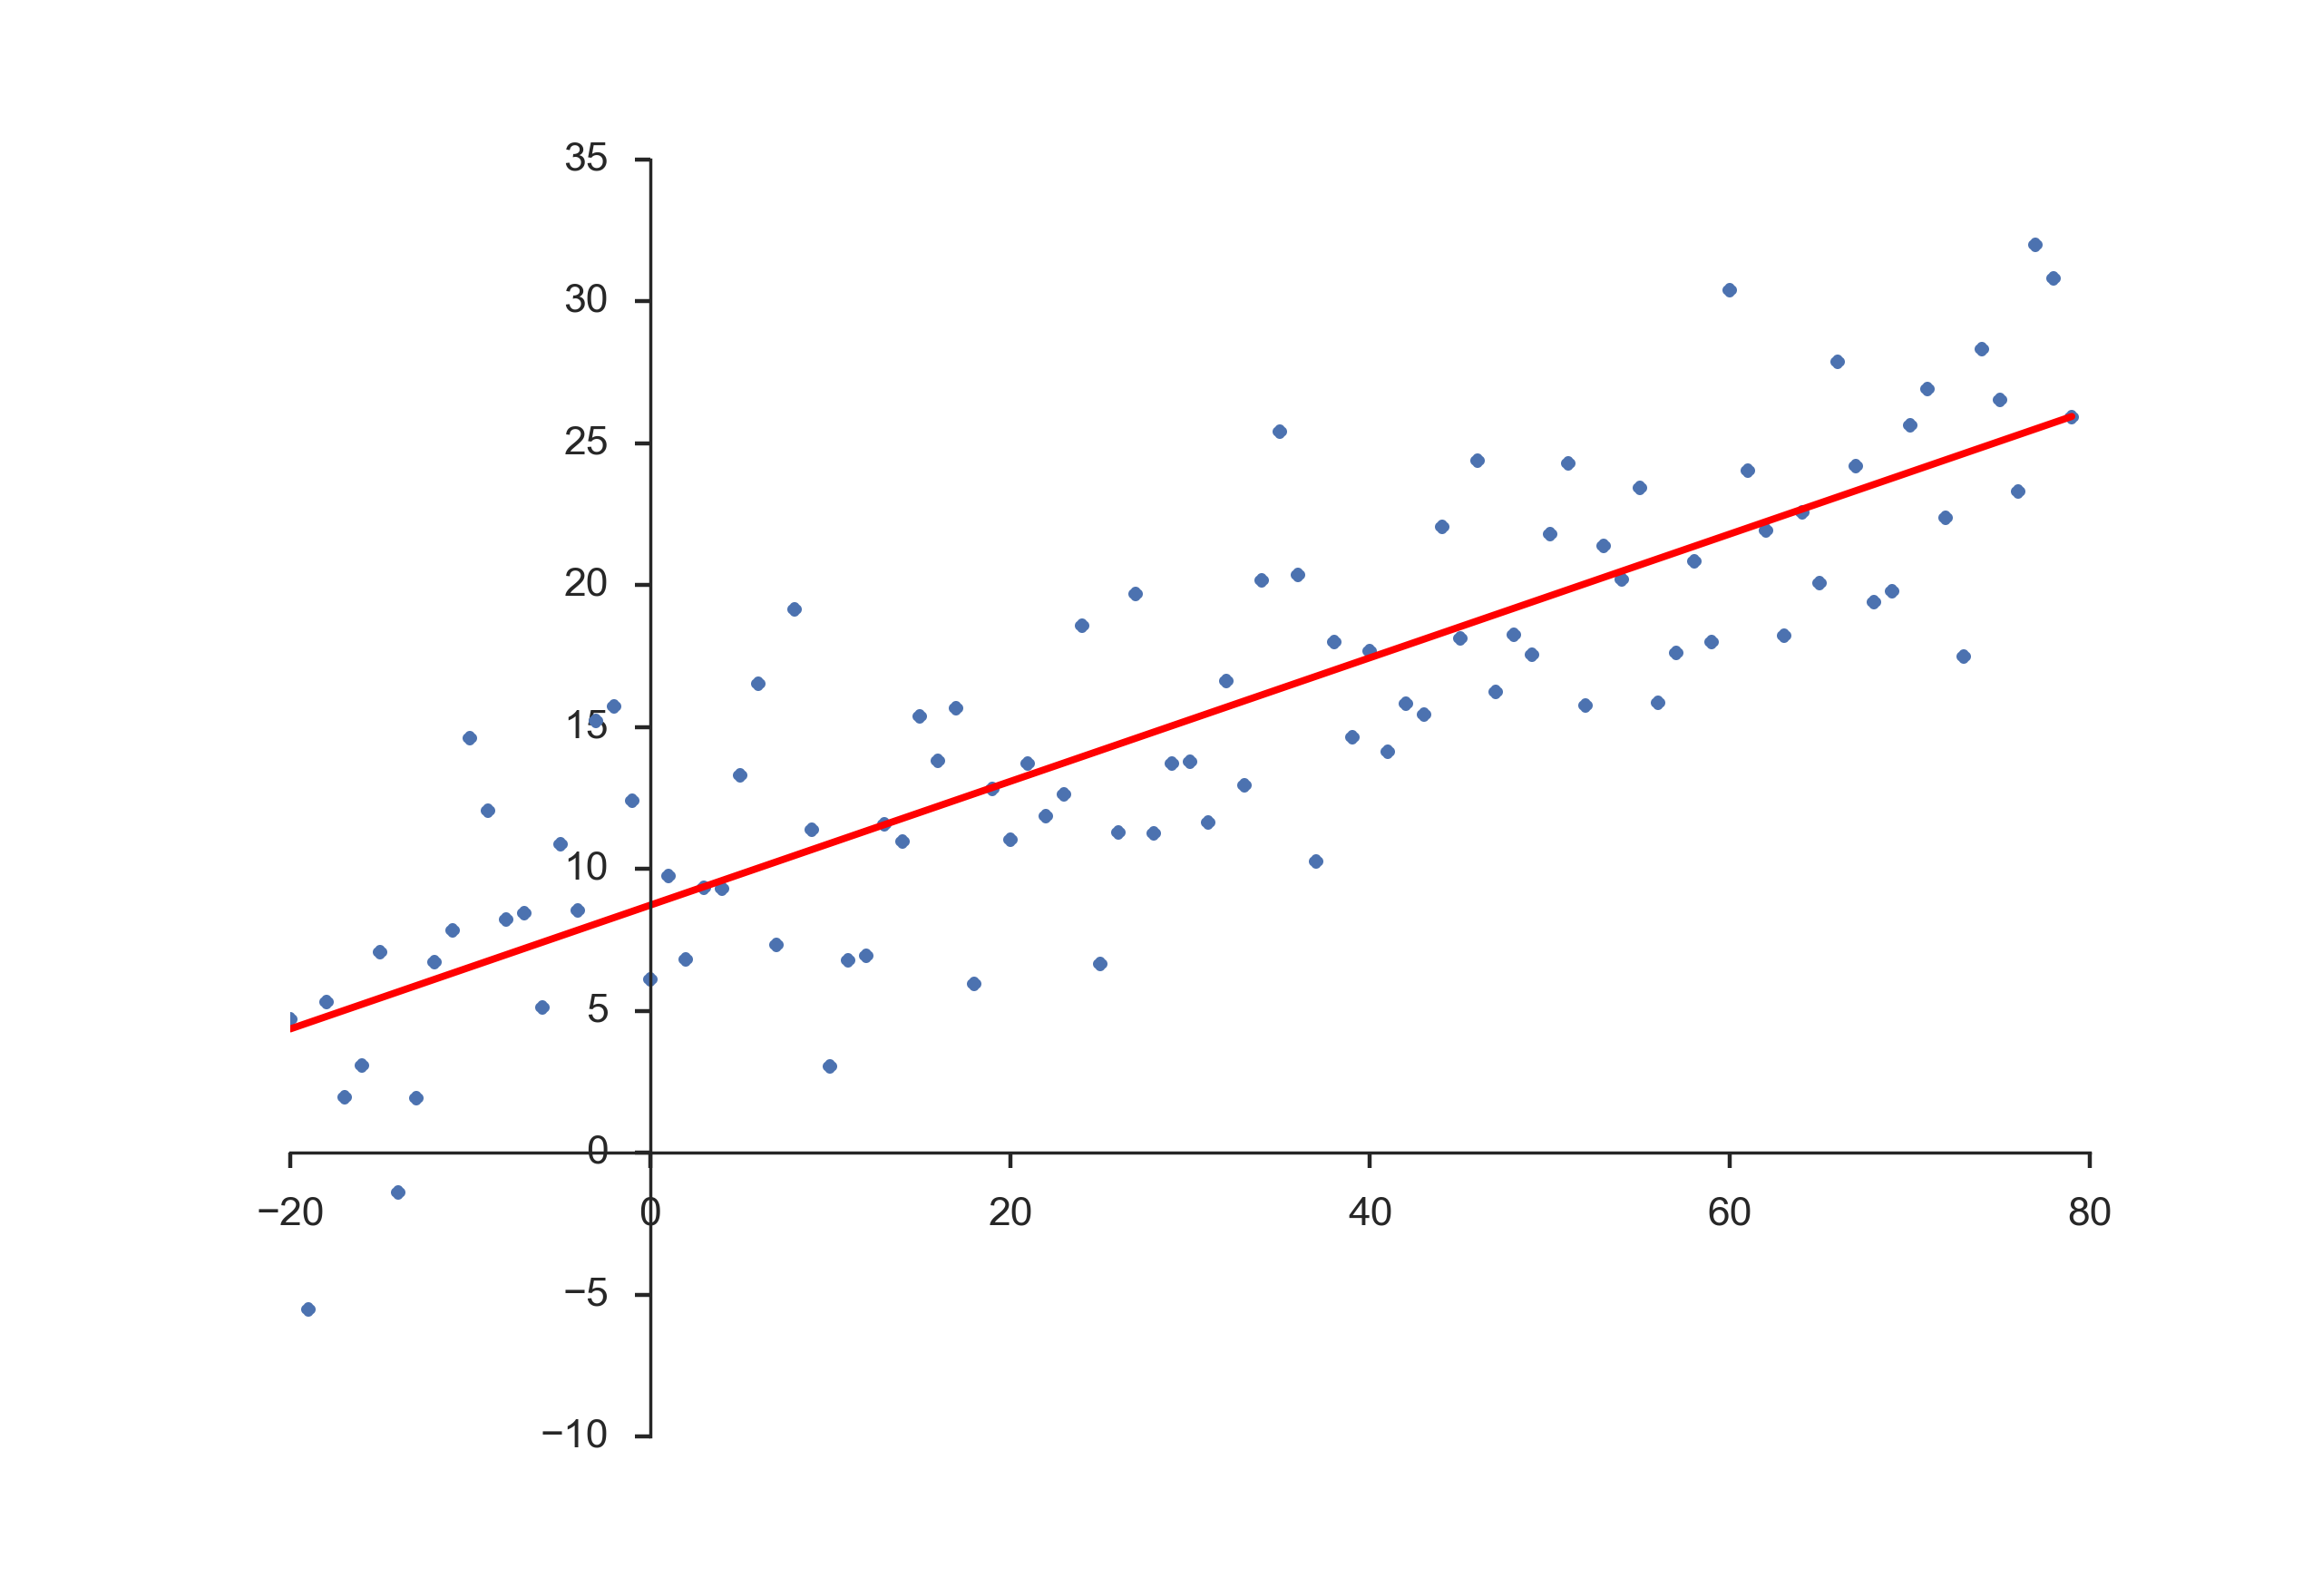
\includegraphics[width=0.75\textwidth]{../Images/Linear_regression.png}\\
  \caption{Linear regression.}\label{fig:regression}
\end{figure}

When we search for the best-fit line to a given $(x_i,y_i)$ data set, we are looking for the parameters $(k,d)$ which minimize the sum of the squared residuals $\epsilon_i$ in

\begin{equation}\label{eq:simpleRegression}
  y_i = k * x_i + d + \epsilon_i
\end{equation}

where $k$ is the slope or inclination of the line, and $d$ the Intercept. This is in fact just the one-dimensional example of the more general technique, which is described in the next section.
Note that in contrast to the correlation, this relationship between $x$ and $y$ is not symmetrical any more: it is assumed that the $x-$values are known exactly, and that all the variability lies in the residuals.

\subsection{Example 1: Simple Linear Regression}

Suppose there are 7 data points $\left\{ {{y_i},{x_i}} \right\}$, where $i=1,2,...,7$. The simple linear regression model is

\begin{equation}
  y_i = \beta_0 + \beta_1 x_i +\epsilon_i, \,
\end{equation}

where $\beta_0$ is the y-intercept and $\beta_1$ is the slope of the regression line. This model can be represented in matrix form as

\begin{equation}\label{eq:simpleRegressionMatrix}
  \begin{bmatrix}y_1 \\ y_2 \\ y_3 \\ y_4 \\ y_5 \\ y_6 \\ y_7 \end{bmatrix}
  =
  \begin{bmatrix}1 & x_1  \\1 & x_2  \\1 & x_3  \\1 & x_4  \\1 & x_5  \\1 & x_6 \\ 1 & x_7  \end{bmatrix}
  \begin{bmatrix} \beta_0 \\ \beta_1  \end{bmatrix}
  +
  \begin{bmatrix} \epsilon_1 \\ \epsilon_2 \\ \epsilon_3 \\ \epsilon_4 \\ \epsilon_5 \\ \epsilon_6 \\ \epsilon_7 \end{bmatrix}
\end{equation}
where the first column of ones in the matrix on the right hand side represents the y-intercept term while the second column is the x-values associated with the y-value.

\subsection{Example 2: Quadratic Fit}

The equation for a quadratic fit to the given data is

\begin{equation}
  y_i = \beta_0 + \beta_1 x_i + \beta_2 x_i^2 +\epsilon_i, \,
\end{equation}

This can be rewritten in matrix form:

\begin{equation}\label{eq:polynomialRegression}
  \begin{bmatrix}y_1 \\ y_2 \\ y_3 \\ y_4 \\ y_5 \\ y_6 \\ y_7 \end{bmatrix}
  =
  \begin{bmatrix}1 & x_1 & x_1^2 \\1 & x_2  & x_2^2 \\1 & x_3  & x_3^2 \\1 & x_4  & x_4^2 \\1 & x_5  & x_5^2 \\1 & x_6  & x_6^2 \\ 1 & x_7  & x_7^2 \end{bmatrix}
  \begin{bmatrix} \beta_0 \\ \beta_1  \\ \beta_2 \end{bmatrix}
  +
  \begin{bmatrix} \epsilon_1 \\ \epsilon_2 \\ \epsilon_3 \\ \epsilon_4 \\ \epsilon_5 \\ \epsilon_6 \\ \epsilon_7 \end{bmatrix}
\end{equation}

% [xxx "the elements of which are assumed to be normally distributed about zero" - is this what the reviewer wanted, when he/she said "No, we also want variance of epsilon" xxx]
\subsection{Coefficient of determination}\label{sec:coeffDetermination}

In order to interpret r, let me first define a few common terms.

\begin{description}
  \item[Residuals] \index{general}{residuals}Differences between observed values and predicted values.
\end{description}

\begin{figure}
  \centering
  \includegraphics[width=0.75\textwidth]{../Images/residuals_linreg.png}\\
  \caption{Best-fit linear regression line (red) and residuals (black). }\label{fig:residuals}
\end{figure}

A data set has values $y_i$, each of which has an associated modelled value $f_i$ (also sometimes referred to as $\hat{y}_i$). Here, the values $y_i$ are called the Observed Values, and the modelled values $f_i$ are sometimes called the Predicted Values.

In the following $\bar{y}$ is the mean of the observed data:

\begin{equation}
  \bar{y}=\frac{1}{n}\sum_{i=1}^n y_i
\end{equation}

where n is the number of observations.

The "variability" of the data set is measured through different sums of squares:
In the following $\hat{y}_i$ will indicate the fitted model values, and $\bar{y}$ will indicate the mean.

\begin{itemize}
  \item $SS_\text{mod} = \sum_{i=1}^n (\hat{y}_i-\bar{y})^2$ is the \emph{Model Sum of Squares}, or the sum of squares for the regression. This value is sometimes also called the Explained Sum of Squares.
  \item $SS_\text{res} = \sum_{i=1}^n (y_i-\hat{y}_i)^2$ is the \emph{Residuals Sum of Squares}, or the sum of squares for the errors.
  \item $SS_\text{tot} = \sum_{i=1}^n (y_i-\bar{y})^2$ is the \emph{Total Sum of Squares}, and is equivalent to the sample variance multiplied by $n-1$.
\end{itemize}

For multiple regression models, $SS_\text{mod} + SS_\text{res} = SS_\text{tot}$

\begin{figure}
  \centering
  \includegraphics[width=0.75\textwidth]{../Images/Coefficient_of_Determination.png}\\
  \caption{The better the linear regression (on the right) fits the data in comparison to the simple average (on the left graph), the closer the value of $R^2$ is to one. The areas of the blue squares represent the squared residuals with respect to the linear regression. The areas of the red squares represent the squared residuals with respect to the average value (from Wikipedia)}\label{fig:CoefDetermination}
\end{figure}


The notations $SS_{R}$ and $SS_{E}$ should be avoided, since in some texts their meaning is reversed to "Residual sum of squares" and "Explained sum of squares", respectively.

With these expressions, the most general definition of the coefficient of determination, $R^2$, is

\begin{equation}\label{eq:R2}
  R^2 \equiv 1 - {SS_{\rm res}\over SS_{\rm tot}}.\,
\end{equation}

Since

\begin{equation}
  SS_\text{tot} = SS_\text{mod} + SS_\text{res}
\end{equation}

Eq. \ref{eq:R2} is equivalent to

\begin{equation}
  R^2 = \frac{SS_\text{mod}}{SS_\text{tot}}
\end{equation}

For simple linear regression (i.e. line-fits), the coefficient of determination\index{general}{coefficient of determination} or $R^2$ is the square of the correlation coefficient $r$. It is easier to interpret than the correlation coefficient r: values of $R^2$ close to 1 are good, values close to 0 are poor.
Note that for general models it is common to write $R^2$, whereas for simple linear regression $r^2$ is used.

\subsubsection{Relation to unexplained variance}\index{general}{unexplained variance}

In a general form, $R^2$ can be seen to be related to the unexplained variance, since the second term in Eq. \ref{eq:R2} compares the unexplained variance (variance of the model's errors) with the total variance (of the data).

\subsubsection{Examples}

How large $R^2$ must be to be considered good depends on the discipline. They are usually expected to be larger in the physical sciences than it is in biology or the social sciences. In finance or marketing, it also depends on what is being modeled.

Caution: the sample correlation and $R^2$ are misleading if there is a nonlinear relationship between the independent and dependent variables!


\section{Model Language}
The mini-language commonly used now in statistics to describe formulas was first used in the languages $R$ and $S$, but is now also available in \emph{Python} through the module \emph{patsy}.

For instance, if we have some variable $y$, and we want to regress it against some other variables $x, a, b$, and the interaction of a and b, then we simply write

\begin{equation}
    y \sim x + a + b + a:b
\end{equation}

This formula language is based on the notation introduced by Wilkinson and Rogers (\cite{Wilkinson1973}, and also used by $S$ and $R$.
The symbols in Table \ref{tab:syntax} are used on the right hand side to denote different interactions.

\begin{table}
  \centering
  \footnotesize{
  \begin{tabular}{ p{2cm} p{9cm} }
     Operator & Meaning \\
     \hline
    $\sim $ &	Separate the left-hand side from the right-hand side. If omitted, formula is assumed right-hand side only. \\
    + &	Combines terms on either side (set union). \\
    - &	Removes terms on the right from set of terms on the left (set difference). \\
    * &	a*b is shorthand for the expansion a + b + a:b. \\
    / &	a/b is shorthand for the expansion a + a:b. It is used when b is nested within a (e.g., states and counties) \\
    : &	Computes the interaction between terms on the left and right. \\
    ** & Takes a set of terms on the left and an integer n on the right and computes the * of that set of terms with itself n times.\\
     \hline
  \end{tabular}
  }
  \caption{Formula syntax}
\end{table}\label{tab:syntax}

A complete set of the description is found under \url{http:\\\\patsy.readthedocs.org}.

\subsection{Design Matrix}

\subsubsection{Definition}
A very general definition of a regression model is the following:

\begin{equation}
  y =f(x,\epsilon)
\end{equation}
In the case of a linear regression model, the model can be rewritten as:

\begin{equation*}
    y=X\beta+ \epsilon,
\end{equation*}

For a simple linear regression and multiple regression, the corresponding Design Matrices are given in \ref{eq:simpleRegressionMatrix} and \ref{eq:multipleRegression}, respectively.

\footnote{This section has been taken from Wikipedia} Given a data set $\{y_i,\, x_{i1}, \ldots, x_{ip}\}_{i=1}^n$ of $n$ statistical units, a linear regression model assumes that the relationship between the dependent variable $y_i$ and the $p$-vector of regressors $x_i$ is linear. This relationship is modelled through a disturbance term or error variable $\epsilon_i$, an unobserved random variable that adds noise to the linear relationship between the dependent variable and regressors. Thus the model takes the form

\begin{equation}\label{eq:regression}
   y_i = \beta_1   x_{i1} + \cdots + \beta_p x_{ip} + \varepsilon_i
   = \mathbf{x}^{\rm T}_i\boldsymbol\beta + \varepsilon_i,
   \qquad i = 1, \ldots, n,
\end{equation}

where $^T$ denotes the transpose, so that $x_i^T\beta$ is the inner product between the vectors $\mathbf{x}_i$ and $\boldsymbol\beta$.

Often these $n$ equations are stacked together and written in vector form as

\begin{equation}
  \mathbf{y} = \mathbf{X}\boldsymbol\beta + \boldsymbol\varepsilon, \,
\end{equation}

where

\begin{equation}
   \mathbf{y} = \begin{pmatrix} y_1 \\ y_2 \\ \vdots \\ y_n \end{pmatrix}, \quad
   \mathbf{X} = \begin{pmatrix} \mathbf{x}^{\rm T}_1 \\ \mathbf{x}^{\rm T}_2 \\ \vdots \\ \mathbf{x}^{\rm T}_n \end{pmatrix}
   = \begin{pmatrix} x_{11} & \cdots & x_{1p} \\
   x_{21} & \cdots & x_{2p} \\
   \vdots & \ddots & \vdots \\
   x_{n1} & \cdots & x_{np}
   \end{pmatrix}, \quad
   \boldsymbol\beta = \begin{pmatrix} \beta_1 \\ \vdots \\ \beta_p \end{pmatrix}, \quad
   \boldsymbol\varepsilon = \begin{pmatrix} \varepsilon_1 \\ \varepsilon_2 \\ \vdots \\ \varepsilon_n \end{pmatrix}.
\end{equation}

Some remarks on terminology and general use:
\begin{itemize} \index{general}{covariate} \index{general}{regressand} \index{general}{endogenous variable} \index{general}{regressor} \index{general}{exogenous variable}
  \item $y_i$  is called the Regressand, Endogenous Variable, Response Variable, Measured Variable, or Dependent Variable.  The decision as to which variable in a data set is modeled as the dependent variable and which are modeled as the independent variables may be based on a presumption that the value of one of the variables is caused by, or directly influenced by the other variables. Alternatively, there may be an operational reason to model one of the variables in terms of the others, in which case there need be no presumption of causality.
  \item $\mathbf{x}_i$ are called Regressors, Exogenous Variables, Explanatory Variables, Covariates, Input Variables, Predictor Variables, or Independent Variables, but not to be confused with Independent Random Variables. The matrix $\mathbf{X}$ is sometimes called the Design Matrix.
      \begin{itemize}
        \item Usually a constant is included as one of the regressors. For example we can take $x_{i1}=1$ for $i=1,...,n$. The corresponding element of $\beta$ is called the Intercept. Many statistical inference procedures for linear models require an intercept to be present, so it is often included even if theoretical considerations suggest that its value should be zero.
        \item Sometimes one of the regressors can be a non-linear function of another regressor or of the data, as in polynomial regression and segmented regression. The model remains linear as long as it is linear in the parameter vector $\beta$ (see Eq. \ref{eq:polynomialRegression}).
         \end{itemize}
  \item $\boldsymbol\beta\,$ is a $p$-dimensional parameter vector. Its elements are also called Effects, or Regression Coefficients. Statistical estimation and inference in linear regression focuses on $\beta$.
  \item $\varepsilon_i\,$ is called the Residuals, Error Term, Disturbance Term, or Noise. This variable captures all other factors which influence the dependent variable $y_i$ other than the regressors $x_i$. The relationship between the error term and the regressors, for example whether they are correlated, is a crucial step in formulating a linear regression model, as it will determine the method to use for estimation.
  \item If $i=1$ and $p=1$ in Eq.\ref{eq:regression}, we have a Simple Linear Regression, corresponding to Eq.\ref{eq:simpleRegression}. If $i>1$ we talk about Multilinear Regression\index{general}{regression!multilinear} or Multiple Linear Regression\index{general}{regression!multiple linear|see{regression!multilinear}} (see Eq. \ref{eq:multipleRegression}).

\end{itemize}

\subsubsection{Examples}

\paragraph{One-way ANOVA (Cell Means Model)}
Example with a one-way analysis of variance (ANOVA) with 3 groups and 7 observations. The given data set has the first three observations belonging to the first group, the following two observations belong to the second group and the final two observations are from the third group.
If the model to be fit is just the mean of each group, then the model is

\begin{equation}
  y_{ij} = \mu_i + \epsilon_{ij}
\end{equation}

which can be written

\begin{equation}
  \begin{bmatrix}y_1 \\ y_2 \\ y_3 \\ y_4 \\ y_5 \\ y_6 \\ y_7 \end{bmatrix} =
  \begin{bmatrix}1 & 0 & 0 \\1 &0  &0 \\ 1 & 0 & 0 \\  0 & 1 & 0 \\  0 & 1 & 0 \\  0 & 0 & 1 \\  0 & 0 & 1\end{bmatrix}
  \begin{bmatrix}\mu_1 \\ \mu_2 \\ \mu_3  \end{bmatrix}
  +
  \begin{bmatrix} \epsilon_1 \\ \epsilon_2 \\ \epsilon_3 \\ \epsilon_4 \\ \epsilon_5 \\ \epsilon_6 \\ \epsilon_7 \end{bmatrix}
\end{equation}
It should be emphasized that in this model $\mu_i$ represents the mean of the $i$th group.

\paragraph{One-way ANOVA (offset from reference group)}
The ANOVA model could be equivalently written as each group parameter $\tau_i$ being an offset from some overall reference.  Typically this reference point is taken to be one of the groups under consideration. This makes sense in the context of comparing multiple treatment groups to a control group and the control group is considered the "reference". In this example, group 1 was chosen to be the reference group. As such the model to be fit is:
\begin{equation}
  y_{ij} = \mu + \tau_i + \epsilon_{ij}
\end{equation}
with the constraint that $\tau_1$ is zero.

\begin{equation}
  \begin{bmatrix}y_1 \\ y_2 \\ y_3 \\ y_4 \\ y_5 \\ y_6 \\ y_7 \end{bmatrix} =
  \begin{bmatrix}1 &0 &0 \\1 &0  &0 \\ 1 & 0 & 0 \\ 1 & 1 & 0 \\ 1 & 1 & 0 \\ 1 & 0 & 1 \\ 1  & 0 & 1\end{bmatrix}
  \begin{bmatrix}\mu \\  \tau_2 \\ \tau_3 \end{bmatrix}
  +
  \begin{bmatrix} \epsilon_1 \\ \epsilon_2 \\ \epsilon_3 \\ \epsilon_4 \\ \epsilon_5 \\ \epsilon_6 \\ \epsilon_7 \end{bmatrix}
\end{equation}
In this model $\mu$ is the mean of the reference group and $\tau_i$ is the difference from group $i$ to the reference group. $\tau_1$ and is not included in the matrix because its difference from the reference group (itself) is necessarily zero.
\subsection{Example: Program Effectiveness}



\PyImg "linRegModel.py" (p \pageref{py:linRegModel}): Estimation of a linear regression model with statsmodels, using the Spector and Mazzeo (1980) data set.
\index{python}{linear regression model}

\section{Linear Regression Analysis with Python}

\subsection{Example 1: Tobacco and Alcohol in the UK}

\footnote{The following is based on the \href{http://connor-johnson.com/2014/02/18/linear-regression-with-python/}{blog of Connor Johnson}.}
We will use \emph{Python} to explore measures of fit for linear regression: the coefficient of determination ($R^2$), hypothesis tests (F, t, Omnibus), AIC, BIC, and other measures.

First we will look at a small data set from \href{http://lib.stat.cmu.edu/DASL/Stories/AlcoholandTobacco.html}{DASL library}, regarding the correlation between tobacco and alcohol purchases in different regions of the United Kingdom. The interesting feature of this data set is that Northern Ireland is reported as an outlier. Notwithstanding, we will use this data set to describe two tools for calculating a linear regression. We will alternatively use the \emph{statsmodels} and \emph{sklearn} modules for calculating the linear regression, while using \emph{pandas} for data management, and \emph{matplotlib} for plotting. To begin, we will import the modules, get the data into \emph{Python}, and have a look at them:

\begin{lstlisting}[language=Python]
    import numpy as np
    import pandas as pd
    import matplotlib.pyplot as plt
    import statsmodels.formula.api as sm
    from sklearn.linear_model import LinearRegression
    from scipy import stats

    data_str = '''Region Alcohol Tobacco
    North 6.47 4.03
    Yorkshire 6.13 3.76
    Northeast 6.19 3.77
    East_Midlands 4.89 3.34
    West_Midlands 5.63 3.47
    East_Anglia 4.52 2.92
    Southeast 5.89 3.20
    Southwest 4.79 2.71
    Wales 5.27 3.53
    Scotland 6.08 4.51
    Northern_Ireland 4.02 4.56'''

    # Read in the data. Note that for \emph{Python} 2.x, you have to change the "import" statement
    from io import StringIO
    df = pd.read_csv(StringIO(data_str), sep=r'\s+')

    # Plot the data
    df.plot('Tobacco', 'Alcohol', style='o')
    plt.ylabel('Alcohol')
    plt.title('Sales in Several UK Regions')
    plt.show()
\end{lstlisting}

\begin{figure}
  \centering
  % Requires \usepackage{graphicx}
  \includegraphics[width=0.5\textwidth]{../Images/Alc_vs_Tobacco.png}\\
  \caption{Sales of Alcohol vs Tobacco in the UK. We notice that there seems to be a linear trend, and one outlier, which corresponds to North Ireland.}
\end{figure}


Fitting the model, leaving the outlier for the moment away is then very easy:

\begin{lstlisting}[language=Python]
    result = smf.ols('Alcohol ~ Tobacco', df[:-1]).fit()
    print(result.summary())
\end{lstlisting}

Note that using the formula API from statsmodels, an intercept is automatically added.  This gives us
\small\begin{lstlisting}[language=Python]

                            OLS Regression Results
==============================================================================
Dep. Variable:                Alcohol   R-squared:                       0.615
Model:                            OLS   Adj. R-squared:                  0.567
Method:                 Least Squares   F-statistic:                     12.78
Date:                Sun, 27 Apr 2014   Prob (F-statistic):            0.00723
Time:                        13:19:51   Log-Likelihood:                -4.9998
No. Observations:                  10   AIC:                             14.00
Df Residuals:                       8   BIC:                             14.60
Df Model:                           1
==============================================================================
                 coef    std err          t      P>|t|      [95.0% Conf. Int.]
------------------------------------------------------------------------------
Intercept      2.0412      1.001      2.038      0.076        -0.268     4.350
Tobacco        1.0059      0.281      3.576      0.007         0.357     1.655
==============================================================================
Omnibus:                        2.542   Durbin-Watson:                   1.975
Prob(Omnibus):                  0.281   Jarque-Bera (JB):                0.904
Skew:                          -0.014   Prob(JB):                        0.636
Kurtosis:                       1.527   Cond. No.                         27.2
==============================================================================
\end{lstlisting}
\normalsize


And now we have a very nice table of mostly meaningless numbers. I will go through and explain each one. The left column of the first table is mostly self explanatory. The degrees of freedom (\emph{Df}) of the model are the number of predictor, or explanatory, variables. The degrees of freedom of the residuals is the number of observations minus the degrees of freedom of the model, minus one (for the offset).

Most of the values listed in the summary are available via the \texttt{result} object. For instance, the $R^2$ value is obtained by \lstinline{result.rsquared}. If you are using \emph{IPython}, you may type \lstinline{result.} and hit the TAB key, and a list of attributes for the \lstinline{result} object will drop down.

\subsection{Model Results}
\subsubsection{Definitions for Regression with Intercept}

$n$ is the number of observations, $k$ is the number of regression parameters. For example, if you fit a straight line, $k=2$.
As above (Chapter \ref{sec:coeffDetermination}) $\hat{y}_i$ will indicate the fitted model values, and $\bar{y}$ will indicate the mean.

\begin{itemize}
  \item $DF_\text{mod} = k - 1$ is the \emph{(Corrected) ModelDegrees of Freedom }. (The "-1" comes from the fact that we are only interested in the correlation, not in the absolute offset of the data.)
  \item $DF_\text{res} = n - k$ is the \emph{Residuals Degrees of Freedom}
  \item $DF_\text{tot} = n - 1$ is the \emph{(Corrected) Total Degrees of Freedom}. The Horizontal line regression is the null hypothesis model.
\end{itemize}

For multiple regression models with intercept, $DF_\text{mod} + DF_\text{res} = DF_\text{tot}$.

\begin{itemize}
  \item $MS_\text{mod} = SS_\text{mod} / DF_\text{mod}$ : \emph{Model Mean of Squares}
  \item $MS_\text{res} = SS_\text{res} / DF_\text{res}$ : \emph{Residuals Mean of Squares}. $MS_\text{res}$ is an unbiased estimate for $\sigma^2$ for multiple regression models.
  \item $MS_\text{tot} = SS_\text{tot} / DF_\text{tot}$ : \emph{Total Mean of Squares}, which is the sample variance of the y-variable.
\end{itemize}

\subsubsection{The $R^2$ Value}

The $R^2$ value indicates the proportion of variation in the y-variable that is due to variation in the x-variables. For simple linear regression, the $R^2$ value is the square of the sample correlation $r_{xy}$. For multiple linear regression with intercept (which includes simple linear regression), the $R^2$ value is defined as

\begin{equation}
  R^2 = \frac{SS_\text{mod}}{SS_\text{tot}}
\end{equation}

\subsection{$\bar{R}^2$ - The \emph{adjusted} $R^2$ Value}\index{general}{coefficient of determination!adjusted}\label{sec:adjustedR2}

Many researchers prefer the \emph{adjusted $\bar{R}^2$ value}, which is penalized for having a large number of parameters in the model:

Here is the logic behind the definition of $\bar{R}^2$:
$R^2$ is defined as $R^2 = 1 - SS_\text{res}/SS_\text{tot}$ or $1 - R^2 = SS_\text{res}/SS_\text{tot}$. To take into account the number of regression parameters $p$, define the \emph{adjusted R-squared} value as
\begin{equation}
  1- \bar{R}^2 = \frac{ResidualVariance }{Total Variance}
\end{equation}

where \emph{(Sample) Residual Variance} is estimated by $SS_\text{res}/DF_\text{res} = SS_\text{res}/(n-k)$, and \emph{(Sample) Total Variance} is estimated by $SS_\text{tot}/DF_\text{tot} = SS_\text{tot}/(n-1)$. Thus,
\begin{eqnarray}
    1 - \bar{R}^2 &=& \frac{SS_\text{res}/(n - k)}{SS_\text{tot}/(n - 1)} \nonumber \\
          	&=& \frac{SS_\text{res}}{SS_\text{tot}}\frac{n - 1}{n - k}
\end{eqnarray}

so

\begin{eqnarray}
  \bar{R}^2 &=& 1 - \frac{SS_\text{res}}{SS_\text{tot}} \frac{n - 1}{n - k} \nonumber  \\
    &=& 1 - (1 - R^2)\frac{n - 1}{n - k}
\end{eqnarray}

\subsubsection{The F-test}

If $t_1, t_2, ... , t_m$ are independent, $N(0, \sigma^2)$ random variables, then $\sum_{i=1}^m \frac{t_i^2}{\sigma^2}$ is a $\chi^2$ (chi-squared) random variable with $m$ degrees of freedom.

For a multiple regression model with intercept,
\begin{equation}
  Y_j = \alpha + \beta_1 X_{1j} + ... + \beta_n X_{nj} + \epsilon_i = \alpha + \sum_{i=1}^n \beta_i X_{ij} + \epsilon_j = E(Y_j | X) + \epsilon_j
\end{equation}

we want to test the following null hypothesis and alternative hypothesis:

        $H_0$:   $\beta_1$ = $\beta_2$ = ... = $\beta_n$ = 0

        $H_1$:   $\beta_j \neq 0$, for at least one value of j

This test is known as the overall \emph{F-test for regression}.

It can be shown that if $H_0$ is true and the residuals are unbiased, homoscedastic (i.e. all function values have the same variance), independent, and normal (see section \ref{sec:Assumptions} ):

\begin{enumerate}
  \item $SS_\text{res} / \sigma^2$ has a $\chi^2$ distribution with $DF_\text{res}$ degrees of freedom.
  \item $SS_\text{mod} / \sigma^2$ has a $\chi^2$ distribution with $DF_\text{mod}$ degrees of freedom.
  \item $SS_\text{res}$ and $SS_\text{mod}$ are independent random variables.
\end{enumerate}

If $u$ is a $\chi^2$ random variable with $n$ degrees of freedom, $v$ is a $\chi^2$ random variable with $m$ degrees of freedom, and $u$ and $v$ are independent, then $F = \frac{u/n}{v/m}$ has an F distribution with $(n,m)$ degrees of freedom.

If H0 is true,

\begin{equation}
  F = \frac{(SS_\text{mod}/\sigma^2)/DF_\text{mod}}{(SS_\text{res}/\sigma^2)/DF_\text{res}} = \frac{SS_\text{mod}/DF_\text{mod}}{SS_\text{res}/DF_\text{res}} = \frac{MS_\text{mod}}{MS_\text{res}},
\end{equation}

has an F distribution with $(DF_\text{mod}, DF_\text{res})$ degrees of freedom, and is independent of $\sigma$.

We can test this directly in \emph{Python} with

\begin{lstlisting}[language=Python]
    N = result.nobs
    k = result.df_model+1
    dfm, dfe = k-1, N - k
    F = result.mse_model / result.mse_resid
    p = 1.0 - stats.f.cdf(F,dfm,dfe)
    print('F-statistic: {:.3f},  p-value: {:.5f}'.format( F, p ))
\end{lstlisting}

which gives us

\begin{lstlisting}[language=Python]
    F-statistic: 12.785,  p-value: 0.00723
\end{lstlisting}

Here, \lstinline{stats.f.cdf( F, m, n )} returns the cumulative sum of the F-distribution with shape parameters \lstinline{m = k-1 = 1}, and \lstinline{n = N - k = 8}, up to the F-statistic $F$. Subtracting this quantity from one, we obtain the probability in the tail, which represents the probability of observing F-statistics more extreme than the one observed.

\subsubsection{Log-Likelihood Function}

A very common approach in statistics is the idea of \gls{maxLikelihood} estimation. \index{general}{Maximum likelihood} The basic idea is quite different from the \emph{least square} approach: there, the model is constant, and the errors of the response are variable; in contrast, in the maximum likelihood approach, the data response values are regarded as constant, and the likelihood of the model is maximised.

For the Classical Linear Regression Model (with normal errors) we have

\begin{equation}
  \epsilon = y_i - \sum_{k=1}^n \beta_k x_{ik} = y_i - \hat{y}_i \; in \; N(0, \sigma^2)
\end{equation}

so the probability density is given by

\begin{equation}
  p(\epsilon_i) =  \Phi (\frac{y_i - \hat{y}_i}{\sigma})
\end{equation}

where $\Phi(z)$ is the standard normal probability distribution function. The probability of independent samples is the product of the individual probabilities

\begin{equation}
  \Pi_{total} = \prod_{i=1}^n p(\epsilon_i)
\end{equation}

The \emph{Log Likelihood function} \index{general}{log likelihood function} is defined as

\begin{eqnarray*}
  ln(\mathfrak{L}) &=& ln(\Pi_{total}) \\
  &=& ln\left[\prod_{i=1}^n \frac{1}{\sigma\sqrt{2 \pi}} \exp \left(\frac{(y_i - \hat{y}_i)^2}{2 \sigma^2}\right)\right] \\
  &=& \sum_{i=1}^n\left[log\left(\frac{1}{\sigma \sqrt{2 \pi}}\right)- \left(\frac{(y_i - \hat{y}_i)^2}{2 \sigma^2}\right)\right]
\end{eqnarray*}

It can be shown that the maximum likelihood estimator of $\sigma^2$ is

\begin{equation}
  E(\sigma^2) = \frac{SS_\text{res}}{n}
\end{equation}

We can calculate this in \emph{Python} as follows:

\begin{lstlisting}[language=Python]
    N = result.nobs
    SSR = result.ssr
    s2 = SSR / N
    L = ( 1.0/np.sqrt(2*np.pi*s2) ) ** N * np.exp( -SSR/(s2*2.0) )
    print('ln(L) =', np.log( L ))

    >>> ln(L) = -4.99975869739

\end{lstlisting}


\subsubsection{Information Content of Statistical Models - AIC and BIC}

% [xxx Is there any way of stating which one is the best? xxx]
To judge the quality of your model, you should first visually inspect the residuals. In addition, you can also use a number of numerical criteria to assess the quality of a statistical model. These criteria represent various approaches for balancing model accuracy with parsimony.

We have already encountered the $adjusted\; R^2$ value (section \ref{sec:adjustedR2}), which - in contrast to the $R^2$ value - decreases if there are too many regressors in the model.

Other commonly encountered criteria are the \emph{Akaike Information Criterion (AIC)} \index{general}{Akaike Information Criterion AIC} and the Schwartz or \emph{Bayesian Information Criterion (BIC)} \index{general}{Bayesian Information Criterion BIC}, which are based on the log-likelihood described in the previous section. Both measures introduce a penalty for model complexity, but the AIC penalizes complexity less severely than the BIC.
The \emph{Akaike Information Criterion AIC} \index{general}{Akaike Information Criterion AIC} is given by

\begin{equation}
  AIC = 2*k - 2*ln(\mathfrak{L})
\end{equation}

and the Schwartz or \emph{Bayesian Information Criterion BIC} \index{general}{Bayesian Information Criterion BIC} by

\begin{equation}
  BIC = k*ln(N) - 2*ln(\mathfrak{L}) .
\end{equation}

Here, $N$ is the number of observations, $k$ is the number of parameters, and $\mathcal{L}$ is the likelihood. We have two parameters in this example, the slope and intercept. The AIC is a relative estimate of information loss between different models. The BIC was initially proposed using a Bayesian argument, and does not relate to ideas of information. Both measures are only used when trying to decide between different models. So, if you have one regression for alcohol sales based on cigarette sales, and another model for alcohol consumption that incorporated cigarette sales and lighter sales, then you would be inclined to choose the model that had the lower AIC or BIC value.

\subsection{Model Coefficients and Their Interpretation}

\subsubsection{Coefficients}
The \emph{coefficients} or weights of the linear regression are contained in \lstinline{result.params}, and returned as a pandas Series object, since we used a pandas DataFrame as input. This is nice, because the coefficients are named for convenience.

\begin{lstlisting}[language=Python]
    result.params
    >>> Intercept    2.041223
    >>> Tobacco      1.005896
    >>> dtype: float64
\end{lstlisting}

We can obtain this directly by computing

\begin{equation}
    \beta = (X^{T}X)^{-1}X^{T}y.
\end{equation}

Here, $X$ is the matrix of predictor variables as columns, with an extra column of ones for the constant term, $y$ is the column vector of the response variable, and $\beta$ is the column vector of coefficients corresponding to the columns of $X$. In \emph{Python}:

\begin{lstlisting}[language=Python]
    df['Eins'] = np.ones(( len(df), ))
    Y = df.Alcohol[:-1]
    X = df[['Tobacco','Eins']][:-1]
\end{lstlisting}


\subsubsection{Standard Error}

% [xxx Check Formulas in Dobson! xxx]
To obtain the \emph{standard errors of the coefficients} we will calculate the covariance-variance matrix, also called the Covariance Matrix, for the estimated coefficients $\beta$ of the predictor variables using

\begin{equation}
    C = cov(\beta) = \sigma^{2} ( X X^{T} )^{-1}.
\end{equation}

Here, $\sigma^{2}$ is the variance, or the MSE (mean squared error) of the residuals. The standard errors are the square roots of the elements on the main diagonal of this covariance matrix. We can perform the operation above, and calculate the element-wise square root using the following \emph{Python} code,

\begin{lstlisting}[language=Python]
    X = df.Tobacco[:-1]

    # add a column of ones for the constant intercept term
    X = np.vstack(( np.ones(X.size), X ))

    # convert the NumPy array to matrix
    X = np.matrix( X )

    # perform the matrix multiplication,
    # and then take the inverse
    C = np.linalg.inv( X * X.T )

    # multiply by the MSE of the residual
    C *= result.mse_resid

    # take the square root
    SE = np.sqrt(C)

    print(SE)

    >>> [[ 0.28132158         nan]
    >>> [        nan  1.00136021]]

\end{lstlisting}

\subsubsection{t-statistic}

We use the t-test to test the null hypothesis that the coefficient of a given predictor variable is zero, implying that a given predictor has no appreciable effect on the response variable. The alternative hypothesis is that the predictor does contribute to the response. In testing we set some threshold, $\alpha = 0.05$, or  0.01, and if $\Pr(T \ge \vert t \vert) \textless \alpha$, then we reject the null hypothesis at our threshold $\alpha$, otherwise we fail to reject the null hypothesis. The t-test generally allows us to evaluate the importance of different predictors, \emph{assuming that the residuals of the model are normally distributed about zero}. If the residuals do not behave in this manner, then that suggests that there is some non-linearity between the variables, and that their t-tests should not be used to assess the importance of individual predictors. Furthermore, it might be best to try to modify the model so that the residuals do tend the cluster normally about zero.

The t statistic is given by the ratio of the coefficient (or factor) of the predictor variable of interest, and its corresponding standard error. If $\beta$ is the vector of coefficients or factors of our predictor variables, and SE is our standard error, then the t statistic is given by,

\begin{equation}
    t_{i} = \beta_{i} / SE_{i,i}
\end{equation}

So, for the first factor, corresponding to the slope in our example, we have the following code,

\begin{lstlisting}[language=Python]
    i = 1
    beta = result.params[i]
    se = SE[i,i]
    t = beta / se
    print('t =', t)

    >>> t = 3.5756084542390316
\end{lstlisting}

Once we have a t statistic, we can (sort of) calculate the probability of observing a statistic at least as extreme as what we have already observed, given our assumptions about the normality of our errors by using the code,

\begin{lstlisting}[language=Python]
    N = result.nobs
    k = result.df_model + 1
    dof = N - k
    p_onesided = 1.0 - stats.t( dof ).cdf( t )
    p = p_onesided * 2.0
    print('p = {0:.3f}'.format(p))

    >>> p = 0.007
\end{lstlisting}

Here, \texttt{dof} are the degrees of freedom, which should be eight, which is the number of observations, N, minus the number of parameters, which is two. The CDF is the cumulative sum of the PDF. We are interested in the area under the right hand tail, beyond our t statistic, t, so we subtract the cumulative sum up to that statistic from one in order to obtain the tail probability on the other side. We then multiply this tail probability by two to obtain a two-tailed probability.

\subsubsection{Confidence Interval}

The confidence interval is built using the standard error, the p-value from our T-test, and a critical value from a T-test having $N-k$ degrees of freedom, where $k$ is the number of observations and $P$ is the number of model parameters, i.e., the number of predictor variables. The confidence interval is the range of values we would expect to find the parameter of interest, based on what we have observed. You will note that we have a confidence interval for the predictor variable coefficient, and for the constant term. A smaller confidence interval suggests that we are confident about the value of the estimated coefficient, or constant term. A larger confidence interval suggests that there is more uncertainty or variance in the estimated term. Again, let me reiterate that hypothesis testing is only one perspective. Furthermore, it is a perspective that was developed in the late nineteenth and early twentieth centuries when data sets were generally smaller and more expensive to gather, and data scientists were using books of logarithm tables for arithmetic.

The confidence interval is given by,

\begin{equation}
    CI =  \beta_{i} \pm z \cdot SE_{i,i}
\end{equation}

Here, $\beta$ is one of the estimated coefficients, $z$ is a \emph{critical-value}, which is the t-statistic required to obtain a probability less than the alpha significance level, and $SE_{i,i}$ is the standard error. The critical value is calculated using the inverse of the cumulative distribution function. (The cumulative distribution function is the cumulative sum of the probability distribution.) In code, the confidence interval using a t-distribution looks like,

\begin{lstlisting}[language=Python]
    i = 0

    # the estimated coefficient, and its variance
    beta, c = result.params[i], SE[i,i]

    # critical value of the t-statistic
    N = result.nobs
    P = result.df_model
    dof = N - P - 1
    z = stats.t( dof ).ppf(0.975)

    # the confidence interval
    print(beta - z * c, beta + z * c)
\end{lstlisting}

\subsection{Analysis of Residuals}

The \textsf{OLS} command from \textsf{statsmodels.formula.api} provides some additional information about the residuals of the model: Omnibus, Skewness, Kurtosis, Durbin-Watson, Jarque-Bera, and the Condition number. In the following we will briefly describe these parameters.

\subsubsection{Skewness and Kurtosis}

Skew and kurtosis refer to the shape of a distribution. \emph{Skewness} is a measure of the asymmetry of a distribution, and \emph{kurtosis} is a measure of its curvature, specifically how pointed the curve is. (For normally distributed data approximately 3.) These values are calculated by hand as

\begin{subequations}
\begin{align}
    S &= \dfrac{\hat{\mu}_{3}}{\hat{\sigma}^{3}} = \dfrac{ \frac{1}{N} \displaystyle \sum_{i=1}^{N} ( y_{i} - \hat{y}_{i} )^{3} }{ \biggl( \frac{1}{N} \displaystyle \sum_{i=1}^{N} ( y_{i} - \hat{y}_{i} )^{2} \biggr)^{3/2}}, \\
    K &= \dfrac{\hat{\mu}_{4}}{\hat{\sigma}^{4}} = \dfrac{ \frac{1}{N} \displaystyle \sum_{i=1}^{N} ( y_{i} - \hat{y}_{i} )^{4} }{ \biggl( \frac{1}{N} \displaystyle \sum_{i=1}^{N} ( y_{i} - \hat{y}_{i} )^{2} \biggr)^{2}}
\end{align}
\end{subequations}


As you see, the $\hat{\mu}_3$ and $\hat{\mu}_4$ are the third and fourth central moments of a distribution. One possible \emph{Python} implementation would be,

\begin{lstlisting}[language=Python]
    d = Y - result.fittedvalues

    S = np.mean( d**3.0 ) / np.mean( d**2.0 )**(3.0/2.0)
    # equivalent to:
    # S = stats.skew(result.resid, bias=True)

    K = np.mean( d**4.0 ) / np.mean( d**2.0 )**(4.0/2.0)
    # equivalent to:
    # K = stats.kurtosis(result.resid, fisher=False, bias=True)
    print('Skewness: {:.3f},  Kurtosis: {:.3f}'.format( S, K ))

    >>> Skewness: -0.014,  Kurtosis: 1.527
\end{lstlisting}

\subsubsection{Omnibus Test}\index{general}{test!Omnibus}

The Omnibus test uses skewness and kurtosis to test the null hypothesis that a distribution is normal. In this case, we’re looking at the distribution of the residual. If we obtain a very small value for $\Pr( \mbox{ Omnibus } )$, then the residuals are not normally distributed about zero, and we should maybe look at our model more closely. The \emph{statsmodels} OLS function uses the \lstinline{stats.normaltest()} function:

\begin{lstlisting}[language=Python]
    (K2, p) = stats.normaltest(result.resid)
    print('Omnibus: {0}, p = {1}'.format(K2, p))

    >>> Omnibus: 2.5418981690649174, p = 0.28056521527106976
\end{lstlisting}

Thus, if either the skewness or kurtosis suggests non-normality, this test should pick it up.

\subsubsection{Durbin-Watson}

The Durbin-Watson test is used to detect the presence of autocorrelation (a relationship between values separated from each other by a given time lag) in the residuals. Here the lag is one.

\begin{equation}
 DW = \dfrac{ \displaystyle \sum_{i=2}^{N} ( ( y_{i} - \hat{y}_i ) - ( y_{i-1} - \hat{y}_{i-1} ) )^{2} }{ \displaystyle \sum_{i=1}^{N} ( y_{i} - \hat{y}_{i} )^{2}}
 \end{equation}

 \begin{lstlisting}[language=Python]
    DW = np.sum( np.diff( result.resid.values )**2.0 ) / result.ssr
    print('Durbin-Watson: {:.5f}'.format( DW ))

    >>> Durbin-Watson: 1.97535
\end{lstlisting}

\subsubsection{Jarque-Bera Test}\index{general}{test!Jarque-Bera}

The Jarque-Bera test is another test that considers skewness (S), and kurtosis (K). The null hypothesis is that the distribution is normal, that both the skewness and excess kurtosis equal zero, or alternatively, that the skewness is zero and the regular run-of-the-mill kurtosis is three. Unfortunately, with small samples the Jarque-Bera test is prone rejecting the null hypothesis -– that the distribution is normal–when it is in fact true.

\begin{equation}
     JB = \dfrac{N}{6} \biggl( S^{2} + \dfrac{1}{4}(K-3)^{2} \biggr)
\end{equation}

Calculating the JB-statistic using the $\chi^{2}$ distribution with two degrees of freedom we have,

\begin{lstlisting}[language=Python]
    JB = (N/6.0) * ( S**2.0 + (1.0/4.0)*( K - 3.0 )**2.0 )
    p = 1.0 - stats.chi2(2).cdf(JB)
    print('JB-statistic: {:.5f},  p-value: {:.5f}'.format( JB, p ))

    >>> JB-statistic: 0.90421,  p-value: 0.63629

\end{lstlisting}

\subsubsection{Condition Number}

The \emph{condition number} \index{general}{condition number} measures the sensitivity of a function's output to its input. When two predictor variables are highly correlated, which is called Multicollinearity\index{general}{multicollinearity}, the coefficients or factors of those predictor variables can fluctuate erratically for small changes in the data, or the model. Ideally, similar models should be similar, i.e., have approximately equal coefficients. Multicollinearity can cause numerical matrix inversion to crap out, or produce inaccurate results. One approach to this problem in regression is the technique of \emph{ridge regression}, which is available in the \texttt{sklearn} \emph{Python} module.

We calculate the condition number by taking the eigenvalues of the product of the predictor variables (including the constant vector of ones) and then taking the square root of the ratio of the largest eigenvalue to the least eigenvalue. If the condition number is greater than thirty, then the regression may have multicollinearity.

\begin{lstlisting}[language=Python]	
    X = np.matrix( X )
    EV = np.linalg.eig( X * X.T )
    print(EV)

    >>> (array([   0.18412885,  136.51527115]), matrix([[-0.96332746, -0.26832855],
    >>> [ 0.26832855, -0.96332746]]))

\end{lstlisting}

Note that $X.T * X$ should be $( P + 1 ) \times ( P + 1 )$, where $P$ is the number of degrees of freedom of the model (the number of predictors) and the +1 represents the addition of the constant vector of ones for the intercept term. In our case, the product should be a $2 \times 2$ matrix, so we’ll have two eigenvalues. Then our condition number is given by,


\begin{lstlisting}[language=Python]	
    CN = np.sqrt( EV[0].max() / EV[0].min() )
    print('Condition No.: {:.5f}'.format( CN ))

    >>> Condition No.: 27.22887
\end{lstlisting}

Our condition number is juuust below 30 (weak!), so we can sort of sleep okay.

\subsection{Comparison}

Now that we have seen an example of linear regression with a reasonable degree of linearity, compare that with an example of one with a significant outlier. In practice, outliers should be understood before they are discarded, because they might turn out to be very important. They might signify a new trend, or some possibly catastrophic event.

\begin{lstlisting}[language=Python]
    X = df[['Tobacco','Eins']]
    Y = df.Alcohol
    result = sm.OLS( Y, X ).fit()
    result.summary()
\end{lstlisting}

\small
\begin{lstlisting}[language=Python]
                            OLS Regression Results
==============================================================================
Dep. Variable:                Alcohol   R-squared:                       0.050
Model:                            OLS   Adj. R-squared:                 -0.056
Method:                 Least Squares   F-statistic:                    0.4735
Date:                Sun, 27 Apr 2014   Prob (F-statistic):              0.509
Time:                        12:58:27   Log-Likelihood:                -12.317
No. Observations:                  11   AIC:                             28.63
Df Residuals:                       9   BIC:                             29.43
Df Model:                           1
==============================================================================
                 coef    std err          t      P>|t|      [95.0% Conf. Int.]
------------------------------------------------------------------------------
Intercept      4.3512      1.607      2.708      0.024         0.717     7.986
Tobacco        0.3019      0.439      0.688      0.509        -0.691     1.295
==============================================================================
Omnibus:                        3.123   Durbin-Watson:                   1.655
Prob(Omnibus):                  0.210   Jarque-Bera (JB):                1.397
Skew:                          -0.873   Prob(JB):                        0.497
Kurtosis:                       3.022   Cond. No.                         25.5
==============================================================================
\end{lstlisting}
\normalsize


\subsection{Example 2: Regression Using Sklearn}

\href{http://scikit-learn.org/}{\emph{Scikit-learn (sklearn)}} \index{general}{scikit-learn} is an open source machine learning library for the \emph{Python} programming language. It features various classification, regression and clustering algorithms.

In order to use \emph{sklearn}, we need to input our data in the form of vertical vectors. Therefore, in our case, we’ll cast the DataFrame to Numpy matrix so that vertical arrays stay vertical once they are sliced off the data set.

\begin{lstlisting}[language=Python]	
    data = np.matrix( df )
\end{lstlisting}

Next, we create the regression objects, and fit the data to them. In this case, we will consider a clean set, which will fit a linear regression better, which consists of the data for all of the regions except Northern Ireland, and an original set consisting of the original data

\begin{lstlisting}[language=Python]	
    cln = LinearRegression()
    org = LinearRegression()

    X, Y = data[:,2], data[:,1]
    cln.fit( X[:-1], Y[:-1] )
    org.fit( X, Y )

    clean_score    = '{0:.3f}'.format( cln.score( X[:-1], Y[:-1] ) )
    original_score = '{0:.3f}'.format( org.score( X, Y ) )
\end{lstlisting}

The next piece of code produces a scatter plot of the regions, with all of the regions plotted as empty blue circles, except for Northern Ireland, which is depicted as a red star.

\begin{lstlisting}[language=Python]
    mpl.rcParams['font.size']=16

    plt.plot( df.Tobacco[:-1], df.Alcohol[:-1], 'bo', markersize=10,
        label='All other regions, $Rˆ2$ = '+clean_score )

    plt.hold(True)
    plt.plot( df.Tobacco[-1:], df.Alcohol[-1:], 'r*', ms=20, lw=10,
        label='N. Ireland, outlier, $Rˆ2$ = '+original_score)
\end{lstlisting}

The next part generates a set of points from 2.5 to 4.85, and then predicts the response of those points using the linear regression object trained on the clean and original sets, respectively.

\begin{lstlisting}[language=Python]
    test = np.arange( 2.5, 4.85, 0.1 )
    test = np.array( np.matrix( test ).T )

    plot( test, cln.predict( test ), 'k' )
    plot( test, org.predict( test ), 'k--' )
\end{lstlisting}

Finally, we limit and label the axes, add a title, overlay a grid, place the legend at the bottom, and then save the figure.

\begin{lstlisting}[language=Python]
    xlabel('Tobacco') ; xlim(2.5,4.75)
    ylabel('Alcohol') ; ylim(2.75,7.0)
    title('Regression of Alcohol from Tobacco')
    grid()
    legend(loc='lower center')
\end{lstlisting}

\begin{figure}
  \centering
  \includegraphics[width=0.75\textwidth]{../Images/alcohol_regressed_over_tobacco.png}
\end{figure}

\subsection{Example 3: Linear Regression Model of a Noisy Quadratic Polynomial}

If you have vectors $x,y$ containing your data, you can use \texttt{statsmodels} to create a design matrix that also includes the $1's$ for the offset:

\begin{lstlisting}[language=Python]
    import statsmodels.api as sm
    Xmat = sm.add_constant(x)
\end{lstlisting}

The parameters are then easily found as

\begin{lstlisting}[language=Python]
    params = np.linalg.lstsq(Xmat, y)
\end{lstlisting}

However, you get a lot more information if you use the OLS-fit from \texttt{statmodels}:

\begin{lstlisting}[language=Python]
    import numpy as np
    import statsmodels.api as sm

    # Generate artificial data
    nobs = 100
    X = np.random.random(nobs)
    X = sm.add_constant(X)
    beta = [5, 3.5]
    e = np.random.random(nobs)
    y = np.dot(X, beta) + e

    # Fit regression model
    results = sm.OLS(y, X).fit()

    # Inspect the results
    print(results.summary())
\end{lstlisting}

yields the following results:

\begin{lstlisting}[language=Python]
                            OLS Regression Results
==============================================================================
Dep. Variable:                      y   R-squared:                       0.923
Model:                            OLS   Adj. R-squared:                  0.922
Method:                 Least Squares   F-statistic:                     1173.
Date:                Fri, 04 Jul 2014   Prob (F-statistic):           2.45e-56
Time:                        14:49:08   Log-Likelihood:                -15.390
No. Observations:                 100   AIC:                             34.78
Df Residuals:                      98   BIC:                             39.99
Df Model:                           1
==============================================================================
                 coef    std err          t      P>|t|      [95.0% Conf. Int.]
------------------------------------------------------------------------------
const          5.4410      0.059     92.685      0.000         5.324     5.557
x1             3.5718      0.104     34.250      0.000         3.365     3.779
==============================================================================
Omnibus:                       21.620   Durbin-Watson:                   2.302
Prob(Omnibus):                  0.000   Jarque-Bera (JB):                5.798
Skew:                           0.223   Prob(JB):                       0.0551
Kurtosis:                       1.908   Cond. No.                         4.60
==============================================================================
\end{lstlisting}

The meaning of many of these parameters is described in the chapter \nameref{chapter:Models}.

From the \texttt{results}, you can extract e.g. the model parameters, standard errors, confidence intervals, and residuals:

\begin{lstlisting}[language=Python]
    params = results.params
    std_err = results.bse
    ConfInt = results.conf_int()
    residuals = results.resid
\end{lstlisting}



\subsection{Conclusion}

Before you do anything, visualize your data. If your data is highly dimensional, then at least examine a few slices using boxplots. At the end of the day, use your own judgement about a model based on your knowledge of your domain. Statistical tests should guide your reasoning, but they should not dominate it. In most cases, your data will not align itself with the assumptions made by most of the available tests. Under \url{http://www.nature.com/news/scientific-method-statistical-errors-1.14700} you can find a very interesting article from Nature on classical hypothesis testing. A more intuitive approach to hypothesis testing is Bayesian analysis.

\section{Assumptions} \label{sec:Assumptions}

To use the technique of linear regression, the following assumptions should be fulfilled:

\begin{enumerate}
  \item The independent variables (i.e. $x$) are exactly known.
  \item Validity. Most importantly, the data you are analyzing should map to the research question you are trying to answer. This sounds obvious but is often overlooked or ignored because it can be inconvenient. For example, a linear regression does not properly describe a quadratic curve.
  \item Additivity and linearity. The most important mathematical assumption of the regression model is that its deterministic component is a linear function of the separate predictors.
  \item Independence of errors from the values of the independent variables.
  \item Equal variance of errors.
  \item Normality of errors.
\end{enumerate}

\begin{figure}
  \centering
  \includegraphics[width=0.75\textwidth]{../Images/Anscombes_quartet.png}\\
  \caption{The sets in the "Anscombe's quartet"\index{general}{Anscombe's quartet} have the same linear regression line but are themselves very different.}
\end{figure}

\PyImg "multivariate.py" (p \pageref{py:multivariate}): Analysis of multivariate data (regression, correlation).
\index{python}{multivariate}

\begin{figure}
  \centering
  \includegraphics[width=0.75\textwidth]{../Images/regression_wLegend.png}\\
  \caption{Regression, with confidence intervals for the mean, as well as for the predicted data. The red dotted line shows the confidence interval for the mean; and the green dotted line the confidence interval for predicted data. (This can be compared to the standard error and the standard deviation for a population.) The corresponding code can be found
  at p. \pageref{py:fitLine}} \label{fig:regline}
\end{figure}

Since to my knowledge there exists no program in the \emph{Python} standard library (or numpy, scipy) to calculate the confidence intervals for a regression line, I include my corresponding program \emph{lineFit.py} \ref{py:fitLine}. The output of this program is shown in Figure \ref{fig:regline}. This program also shows how \emph{Python} programs intended for distribution should be documented.

\PyImg "fitLine.py" (p \pageref{py:fitLine}): Linear regression fit.
\index{python}{fitLine}




Standard linear regression models with standard estimation techniques make a number of assumptions about the predictor variables, the response variables and their relationship.  Numerous extensions have been developed that allow each of these assumptions to be relaxed (i.e. reduced to a weaker form), and in some cases eliminated entirely.  Some methods are general enough that they can relax multiple assumptions at once, and in other cases this can be achieved by combining different extensions.  Generally these extensions make the estimation procedure more complex and time-consuming, and may also require more data in order to get an accurate model.

The following are the major assumptions made by standard linear regression models with standard estimation techniques (e.g. ordinary least squares):

\begin{itemize}
  \item \textbf{Weak exogeneity}.  This essentially means that the predictor variables $x$ can be treated as fixed values, rather than random variables.  This means, for example, that the predictor variables are assumed to be error-free, that is they are not contaminated with measurement errors. Although not realistic in many settings, dropping this assumption leads to significantly more difficult errors-in-variables models.

  \item \textbf{Linearity}.  This means that the mean of the response variable is a linear combination of the parameters (regression coefficients) and the predictor variables.  Note that this assumption is much less restrictive than it may at first seem.  Because the predictor variables are treated as fixed values (see above), linearity is really only a restriction on the parameters.  The predictor variables themselves can be arbitrarily transformed, and in fact multiple copies of the same underlying predictor variable can be added, each one transformed differently.  This trick is used, for example, in polynomial regression, which uses linear regression to fit the response variable as an arbitrary polynomial function (up to a given rank) of a predictor variable. This makes linear regression an extremely powerful inference method.  In fact, models such as polynomial regression are often "too powerful", in that they tend to overfit the data.  As a result, some kind of regularization must typically be used to prevent unreasonable solutions coming out of the estimation process.  Common examples are ridge regression and lasso regression.  Bayesian linear regression can also be used, which by its nature is more or less immune to the problem of overfitting. (In fact, ridge regression and lasso regression can both be viewed as special cases of Bayesian linear regression, with particular types of prior distributions placed on the regression coefficients.)

  \item \textbf{Constant variance} (aka \emph{homoscedasticity})\index{general}{homoscedasticity}.  This means that different response variables have the same variance in their errors, regardless of the values of the predictor variables. In practice this assumption is invalid (i.e. the errors are heteroscedastic) if the response variables can vary over a wide scale. In order to determine for heterogeneous error variance, or when a pattern of residuals violates model assumptions of homoscedasticity (error is equally variable around the 'best-fitting line' for all points of x), it is prudent to look for a "fanning effect" between residual error and predicted values. This is to say there will be a systematic change in the absolute or squared residuals when plotted against the predicting outcome. Error will not be evenly distributed across the regression line. Heteroscedasticity will result in the averaging over of distinguishable variances around the points to get a single variance that is inaccurately representing all the variances of the line. In effect, residuals appear clustered and spread apart on their predicted plots for larger and smaller values for points along the linear regression line, and the mean squared error for the model will be wrong. Typically, for example, a response variable whose mean is large will have a greater variance than one whose mean is small. For example, a given person whose income is predicted to be \$100,000 may easily have an actual income of \$80,000 or \$120,000 (a standard deviation]] of around \$20,000), while another person with a predicted income of \$10,000 is unlikely to have the same \$20,000 standard deviation, which would imply their actual income would vary anywhere between -\$10,000 and \$30,000. (In fact, as this shows, in many cases – often the same cases where the assumption of normally distributed errors fails – the variance or standard deviation should be predicted to be proportional to the mean, rather than constant.) Simple linear regression estimation methods give less precise parameter estimates and misleading inferential quantities such as standard errors when substantial heteroscedasticity is present. However, various estimation techniques (e.g. weighted least squares and heteroscedasticity-consistent standard errors) can handle heteroscedasticity in a quite general way. Bayesian linear regression techniques can also be used when the variance is assumed to be a function of the mean. It is also possible in some cases to fix the problem by applying a transformation to the response variable (e.g. fit the logarithm of the response variable using a linear regression model, which implies that the response variable has a log-normal distribution rather than a normal distribution).

  \item \textbf{Independence of errors}.  This assumes that the errors of the response variables are uncorrelated with each other. (Actual statistical independence is a stronger condition than mere lack of correlation and is often not needed, although it can be exploited if it is known to hold.) Some methods (e.g. generalized least squares) are capable of handling correlated errors, although they typically require significantly more data unless some sort of regularization is used to bias the model towards assuming uncorrelated errors. Bayesian linear regression is a general way of handling this issue.

  \item \textbf{Lack of multicollinearity in the predictors}.  For standard least squares estimation methods, the design matrix $X$ must have full column rank $p$; otherwise, we have a condition known as multicollinearity in the predictor variables.  This can be triggered by having two or more perfectly correlated predictor variables (e.g. if the same predictor variable is mistakenly given twice, either without transforming one of the copies or by transforming one of the copies linearly). It can also happen if there is too little data available compared to the number of parameters to be estimated (e.g. fewer data points than regression coefficients). In the case of multicollinearity, the parameter vector $\beta$ will be non-identifiable, it has no unique solution.  At most we will be able to identify some of the parameters, i.e. narrow down its value to some linear subspace of $R^p$. Methods for fitting linear models with multicollinearity have been developed. Note that the more computationally expensive iterated algorithms for parameter estimation, such as those used in generalized linear models, do not suffer from this problem — and in fact it's quite normal to when handling categorical data|categorically-valued predictors to introduce a separate indicator variable predictor for each possible category, which inevitably introduces multicollinearity.
\end{itemize}

Beyond these assumptions, several other statistical properties of the data strongly influence the performance of different estimation methods:

\begin{itemize}
  \item The statistical relationship between the error terms and the regressors plays an important role in determining whether an estimation procedure has desirable sampling properties such as being unbiased and consistent.
  \item The arrangement, or probability distribution of the predictor variables $x$ has a major influence on the precision of estimates of $\beta$. Sampling and design of experiments are highly-developed subfields of statistics that provide guidance for collecting data in such a way to achieve a precise estimate of $\beta$.
\end{itemize}

\subsection{Interpretation}

A fitted linear regression model can be used to identify the relationship between a single predictor variable $x_j$ and the response variable $y$ when all the other predictor variables in the model are “held fixed”. Specifically, the interpretation of $\beta_j$ is the expected change in $y$ for a one-unit change in $x_j$ when the other covariates are held fixed—that is, the expected value of the partial derivative of $y$ with respect to $x_j$. This is sometimes called the Unique Effect of $x_j$ on "y". In contrast, the Marginal Effect of $x_j$ on $y$ can be assessed using a correlation coefficient or simple linear regression model relating $x_j$ to $y$; this effect is the total derivative of $y$ with respect to $x_j$.

Care must be taken when interpreting regression results, as some of the regressors may not allow for marginal changes (such as dummy variables, or the intercept term), while others cannot be held fixed (recall the example from the introduction: it would be impossible to “hold $t_j$ fixed” and at the same time change the value of $t_i^2$.

It is possible that the unique effect can be nearly zero even when the marginal effect is large. This may imply that some other covariate captures all the information in $x_j$, so that once that variable is in the model, there is no contribution of $x_j$ to the variation in $y$. Conversely, the unique effect of $x_j$ can be large while its marginal effect is nearly zero. This would happen if the other covariates explained a great deal of the variation of $y$, but they mainly explain variation in a way that is complementary to what is captured by $x_j$. In this case, including the other variables in the model reduces the part of the variability of $y$ that is unrelated to $x_j$, thereby strengthening the apparent relationship with $x_j$.

The meaning of the expression “held fixed” may depend on how the values of the predictor variables arise. If the experimenter directly sets the values of the predictor variables according to a study design, the comparisons of interest may literally correspond to comparisons among units whose predictor variables have been “held fixed” by the experimenter. Alternatively, the expression “held fixed” can refer to a selection that takes place in the context of data analysis. In this case, we “hold a variable fixed” by restricting our attention to the subsets of the data that happen to have a common value for the given predictor variable. This is the only interpretation of “held fixed” that can be used in an observational study.

The notion of a “unique effect” is appealing when studying a complex system where multiple interrelated components influence the response variable. In some cases, it can literally be interpreted as the causal effect of an intervention that is linked to the value of a predictor variable. However, it has been argued that in many cases multiple regression analysis fails to clarify the relationships between the predictor variables and the response variable when the predictors are correlated with each other and are not assigned following a study design.

\PyImg "modeling.py" (p \pageref{py:modeling}) shows an example.
\index{python}{modeling}

\section{Bootstrapping} \index{general}{bootstrapping}

Another type of modelling is \emph{bootstrapping}. Sometimes you have data describing a distribution, but do not know what type of distribution it is. So what can you do if you want to find out e.g. confidence values for the mean?

The answer is bootstrapping. Bootstrapping is a scheme of \emph{resampling}, i.e. taking additional samples repeatedly from the initial sample, to provide estimates of its variability. In a case where the distribution of the initial sample is unknown, bootstrapping is of especial help in that it provides information about the distribution.

\PyImg "bootstrapDemo.py" (p \pageref{py:bootstrapDemo}): Example of bootstrapping the confidence interval for the mean of a sample distribution.
\index{python}{bootstrapDemo}
\section{Exercises}

\begin{enumerate}
  \item \textbf{Correlation}

    Read in the data for the average yearly temperature at the Sonnblick, from     \emph{https://github.com/thomas-haslwanter/statsintro/blob/master/Data/data\_others/AvgTemp.xls}
    Calculate the Pearson and Spearman correlation, and Kendall's tau, for the temperature vs. year.

  \item \textbf{Regression}

    For the same data, calculate the yearly increase in temperature, assuming a linear increase with time.
    Is this increase significant?

  \item \textbf{Normality Check}

    For the data from the regression model, check if the model is ok by testing if the residuals are normally distributed (e.g. by using the Kolmogorov-Smirnov test)

\end{enumerate}


